\documentclass[10pt, a4paper, twocolumn]{article}
\usepackage{lipsum}
\usepackage[english]{babel}
\usepackage{fancyhdr}
\usepackage{geometry}
\usepackage{graphicx}
\usepackage[T1]{fontenc}
\usepackage{uarial}
\usepackage{indentfirst}
\usepackage[font=small]{caption}
\usepackage{xcolor}
\usepackage{dblfloatfix}
\usepackage{biblatex}

\addbibresource{refs_ciicusp.bib}


\renewcommand{\familydefault}{\sfdefault}
\geometry{a4paper, left=2.6cm, right=2.6cm, bottom=4.2cm, headheight=1.35cm, top=3.4cm}
\setlength{\columnsep}{0.8cm}
\pagestyle{fancy}
\fancyhf{} 
\lhead{
\includegraphics[width=1.6cm]{figures/siicusp.png}}
\renewcommand{\headrulewidth}{0pt}



\begin{document}

\twocolumn[%
  \begin{center}
    {\bf\fontsize{13}{16}\selectfont MORPHOLOGICAL CLASSIFICATION OF S-PLUS GALAXIES USING A ENSEMBLE OF CONVOLUTIONAL NEURAL NETWORK\\[13pt]}

    {\bf\fontsize{13}{16}\selectfont Natanael Magalhães Cardoso\\[13pt]}

    {\bf\fontsize{13}{16}\selectfont Profa. Cláudia Mendes de Oliveira\\[13pt]}

    {\fontsize{13}{16}\selectfont Instituto de Astronomia, Geofísica e Ciências Atmosféricas, USP -- SP\\[13pt]}

    {\fontsize{10}{12}\selectfont nauxmac@gmail.com}

    \vspace{39pt}
  \end{center}
]


\begin{center}
  \bf\fontsize{13}{15.6}\selectfont Objectives
\end{center}

Morphological classification is the cataloging of galaxies according to their visual appearance and it is linked to their physical properties. A morphological classification made through visual analysis is sensible to differences in evaluation among diferent human volunteers. For this reason, systematic, objective and easily reproducible classification of galaxies has been gaining importance since the astronomer Edwin Hubble created his famous classification method \cite{hubble1926}. In this work, we combine accurate visual classifications of the GalaxyZoo\footnote{http://galaxyzoo.org} project with Deep Learning methods. The goal is to find an automatic and efficient technique at human performance level classification based on analysis of DR1 images of the Southern Photometric Local Universe Survey (S-PLUS) \cite{oliveira2019} and publish a catalog with not yet classified galaxies. For this, a Deep Learning model was developed through a set of four convolutional neural networks using the Stacking Ensemble technique \cite{Wolpert1992}.

\begin{center}
  \bf\fontsize{13}{15.6}\selectfont Materials and Methods
\end{center}

\begin{figure*}[!h]
  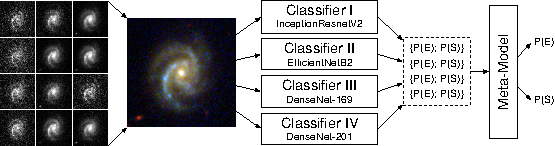
\includegraphics[width=\textwidth]{figures/arch_en.pdf}
  \caption{Architecture diagram. From left to right, the 12 images of each band are grouped into a single RGB image, which is the input for the individual classifiers. These classifiers have the function of extracting visual features from the image and returning the probability of being elliptical or spiral. The metamodel has the function of combining the predictions of the classifiers into a single, more robust prediction.}
  \label{fig:arch}
\end{figure*}

The proposed model classifies the morphology of galaxies based on their images. The images of each of the 12 bands (details about each band in Table 1 of \cite{oliveira2019}) were obtained from the S-PLUS project database\footnote{http://splus.cloud}, grouped in 3 bands and converted to RGB color space. This reduction step allows the use of the information from the 12 bands, mapped into only 3 bands, causing a reduction in the training time of the models. As the proposed technique consists of a supervised training, in addition to the data to be classified, GalaxyZoo human classifications are also necessary so that the algorithm can relate the patterns between the images and their respective classes. The training, validation and testing sets were created, with approximately 30\% of elliptical galaxies and 70\% of spiral galaxies. Techniques such as random resampling and class weighting were used to address the imbalance. Another set, called \emph{blind}, was created with galaxies not yet classified by GalaxyZoo and which will be classified by the model. All these sets have similar redshift distribution and magnitude.


To train the classifiers, convolutional neural networks with weights initialized from a pre-training on ImageNet\footnote{http://image-net.org} were used. The data pre-processing, the hyperparameter adjustment and the training were done for each classifier independently. Among the trained models, the ones that obtained the best classification performance are based on the InceptionResNetV2, EfficientNetB2, DenseNet-169 and DenseNet-201 architectures. To take full advantage of the potential of these four classifiers, another model (called meta-model) was trained to receive the predictions of each classifier and return a single prediction. Thus, a Ensemble of classifiers is formed. This procedure is summarized in the diagram in Figure \ref{fig:arch}.

\break
\begin{center}
  \bf\fontsize{13}{15.6}\selectfont Results
\end{center}

\begin{figure}[!b]
  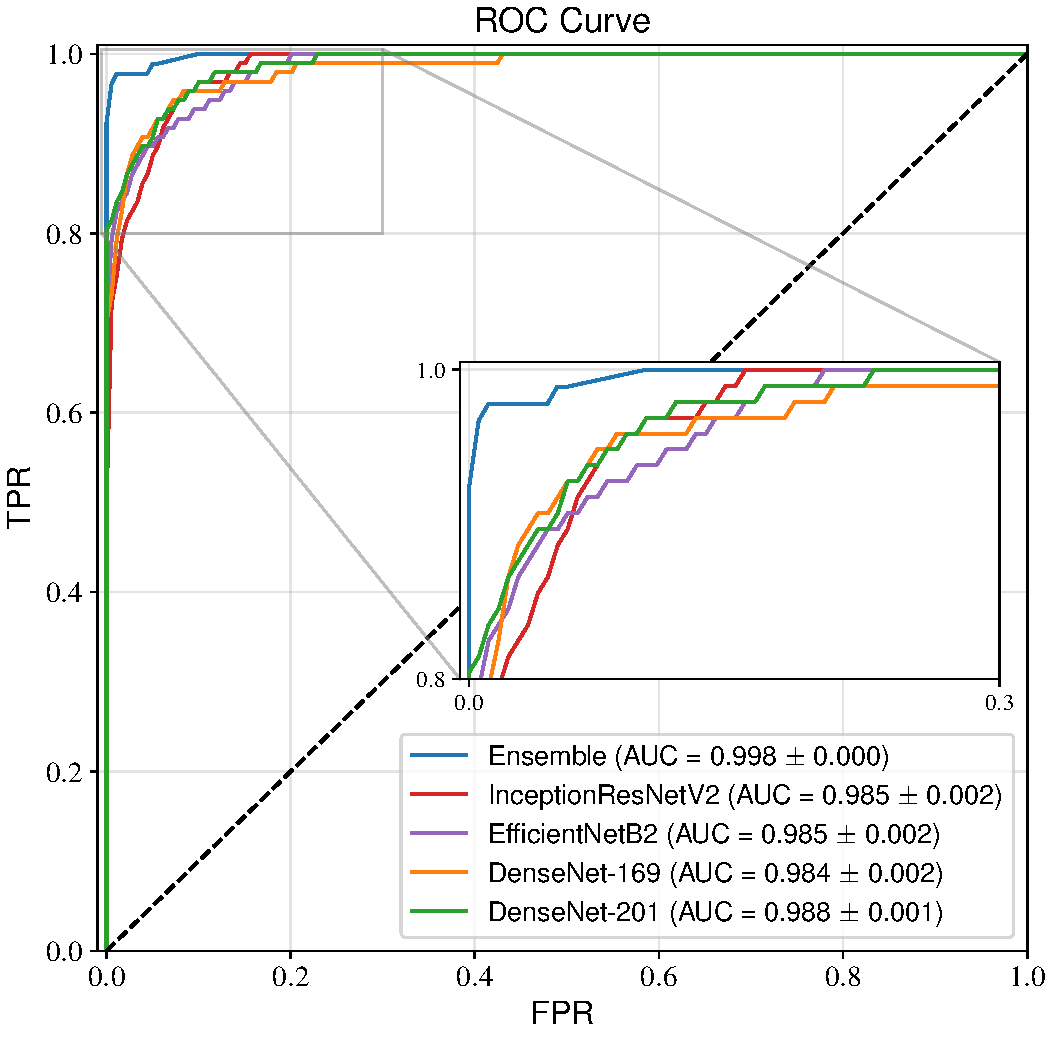
\includegraphics[width=\linewidth]{figures/roc_mn170_en.pdf}
  \caption{ROC curve for each classifier and for the Ensemble. Each curve represents the median of 60 measurements, the area under the curve (AUC) and its standard deviation are in the legend for each curve.}
  \label{fig:roc}
\end{figure}

One way to evaluate the model quantitatively is from the Receiver Operating Characteristic Curve (ROC) in the test set, as shown in Figure \ref{fig:roc}. From this graph it is possible to draw conclusions about the classification potential of the model. The area under the curve, whose maximum value is 1, indicates the probability of correct classification by the model. Furthermore, the faster the curve reaches the top, the greater the degree of separability of the model, that is, the greater the model's ability to distinguish between classes. As expected, the Ensemble (blue curve), which is the union of the four classifiers, outperforms the individual classifiers, reaching an AUC of 0.998.

\begin{center}
  \bf\fontsize{13}{15.6}\selectfont Conclusions
\end{center}

From this project, a fully developed and operational Deep Learning model was obtained with high potential for morphological classification between elliptical and spiral galaxies from S-PLUS images, as well as a catalog with automated classifications of 2536 galaxies with magnitude less than 17 without classifications on GalaxyZoo, both publicly available\footnote{http://natanael.net}. In addition, a scientific paper about this project is in the final writing stages.


\begin{center}
  \bf\fontsize{13}{15.6}\selectfont References
\end{center}

\printbibliography[heading=none]


\end{document}